\begin{wrapfigure}[20]{r}{0.5\linewidth}
\centering
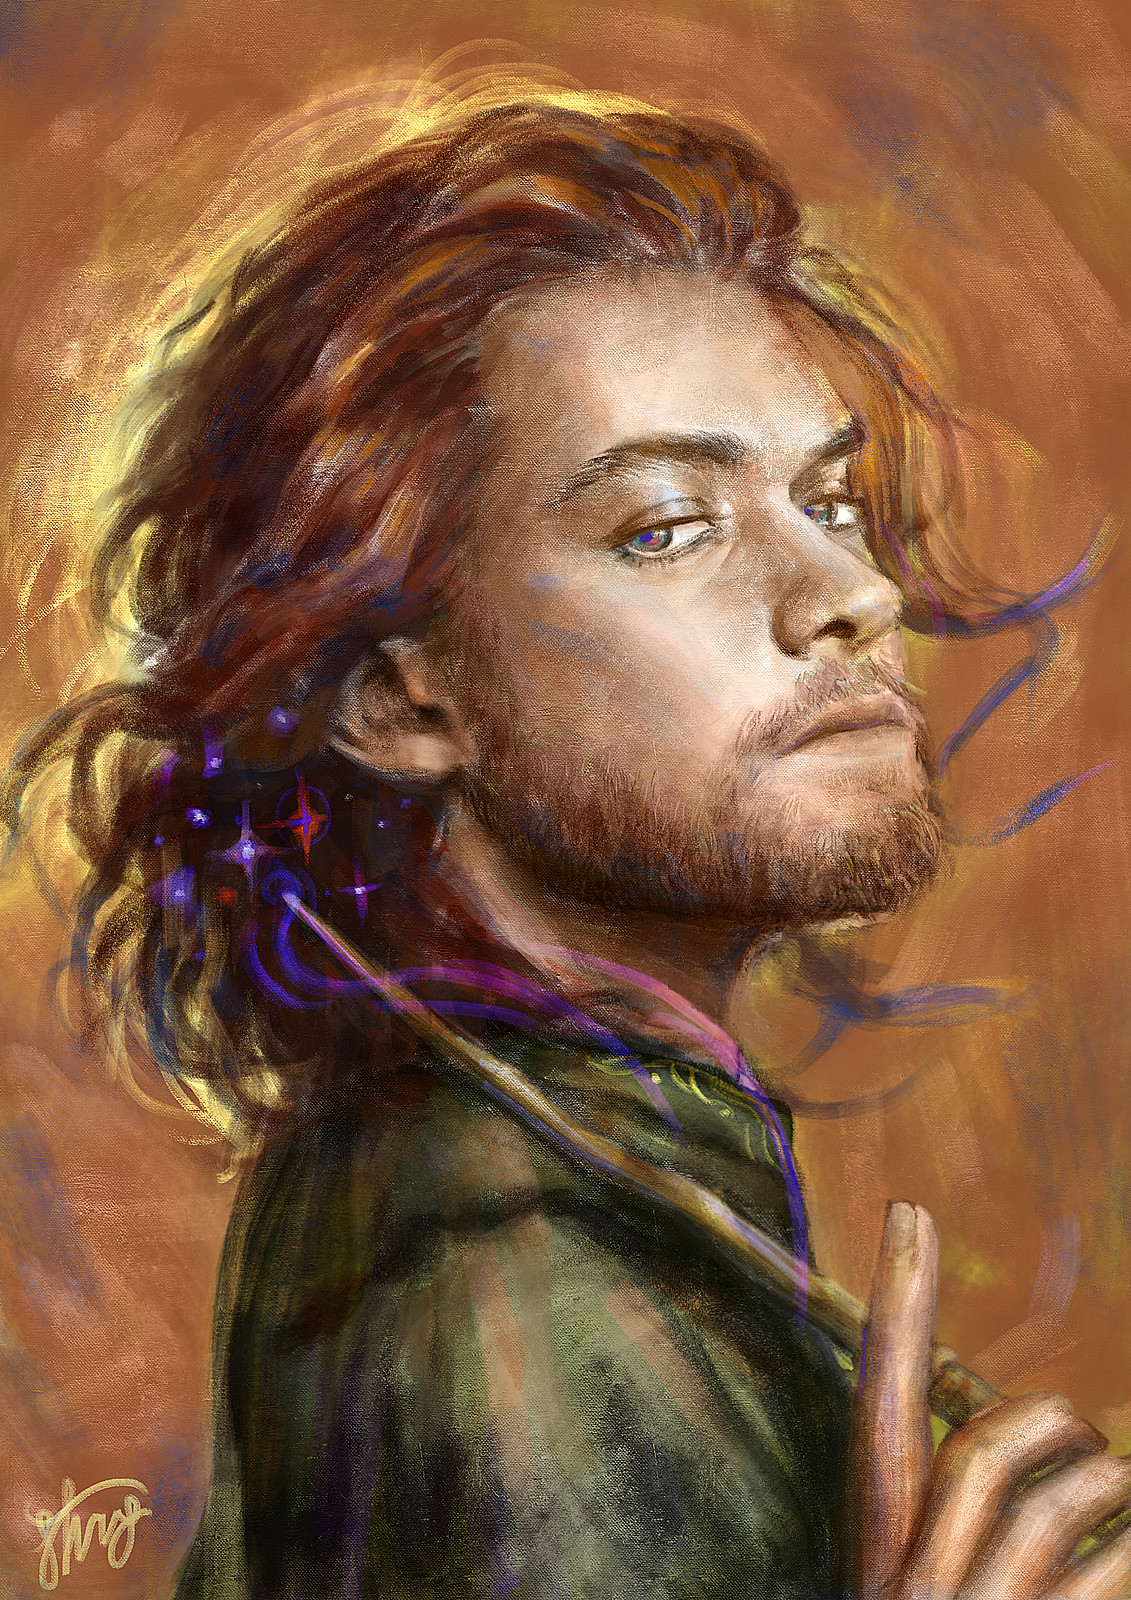
\includegraphics[max width=0.5\textwidth]{../Pictures/Characters/Portraits/Albus_portrait.png}
\end{wrapfigure}

\paragraph{Description}
Albus Percival Wulfric Brian Dumbledore is an auburn-haired half-blood wizard.

He is currently teaching at Hogwarts: formerly a Defense against the Dark Arts professor, now presides over the Transfiguration class. Amongst its students we can find the proficient Minerva McGonagall, with whom he had developed a friendly mentorship, the eerie but clever Tom Riddle and the newcomer Delphini Lestrange, which sparked some suspicions because of her unusual arrival.

\paragraph{Backstory}
Albus childhood was marked by tragedy by the attack of some muggle boys on her sister Ariana, who saw her performing magic and were frightened by what they saw. Some anti-muggle prejudice did develop in his early years, especially when he was in his relationship with Gellert Grindelwald, however he soon saw the error of his intent and changed his mind. This lead him to break his relationship with Grindelwald, followed by such a violent discussion that her sister Ariana was killed while trying to stop their fight. 

From that experience, Albus changed completely, repudiating any possible anti-muggle or mage-elitist movement and fighting against them.

\begin{figure}[H]
\includegraphics[max width=\textwidth]{../Pictures/Characters/Circumplexes/Albus_circumplex.png} 
\captionsetup{labelformat=empty}
\caption{Circumplex}
\end{figure}

\begin{figure}[H]
\includegraphics[max width=\textwidth]{../Pictures/Characters/Relationship_maps/Albus_relmap.png} 
\captionsetup{labelformat=empty}
\caption{Map of relationships at the start of the game}
\includegraphics[max width=\textwidth]{../Pictures/Characters/Relationship_maps/Albus_after_event_relmap.png} 
\captionsetup{labelformat=empty}
\caption{Map of relationships after Delphini changes her mind thanks to Minerva's friendship}
\end{figure}


\clearpage